%++++++++++++++++++++++++++++++++++++++++
% Don't modify this section unless you know what you're doing!
\documentclass[letterpaper,12pt]{article}
\usepackage{tabularx} % extra features for tabular environment
\usepackage{amsmath}  % improve math presentation
\usepackage{graphicx} % takes care of graphic including machinery
\usepackage[margin=1in,letterpaper]{geometry} % decreases margins
\usepackage{cite} % takes care of citations
\usepackage[utf8]{inputenc}
\usepackage[final]{hyperref} % adds hyper links inside the generated pdf file
\hypersetup{
	colorlinks=true,       % false: boxed links; true: colored links
	linkcolor=blue,        % color of internal links
	citecolor=blue,        % color of links to bibliography
	filecolor=magenta,     % color of file links
	urlcolor=blue
}
%++++++++++++++++++++++++++++++++++++++++
\newcommand{\code}[1]{\texttt{#1}}
\renewcommand*{\arraystretch}{1.2}
\setlength{\parindent}{0cm}

\begin{document}

\title{Programming Assignment}
\author{Miguel Alcón Doganoc}
\date{\today}
\maketitle

\section{Introduction}
The objective of this assignment is to do an empirical comparison of the computing time that the algorithms \textbf{QSelect}, \textbf{RMedian}, \textbf{QuickSort} and \textbf{MergeSort} need to find the median of an array of numbers. Being \textbf{QuickSort} and \textbf{MergeSort} sorting algorithms, finding the median means sorting the array and going to the position $\lceil n/2 \rceil $. We have that:
\begin{itemize}
    \item Quick select or \textbf{QSelect} takes $O(n)$ in expectation.
    \item Randomized median or \textbf{Rmedian} takes $O(n)$ in expectation.
    \item Merge sort or \textbf{MergeSort} takes $O(n \log n)$.
    \item Quick sort or \textbf{QuickSort} takes $O(n \log n)$ in average.
\end{itemize}

\section{Algorithm Implementation}
I used \textit{Python 3} to make the implementation of the whole experiment. I have written all the code, but I have inspired by some algorithms on Internet. The implementations of \textbf{QSelect} and \textbf{Mergesort} where inspired by \cite{qselect} and \cite{mergesort}, respectively, but they have some modifications made by me. My implementation of \textbf{QuickSort} is based on the \textbf{QSelect} implementation and what I know about the algorithm. I want to mention that the pivot of my \textbf{QuickSort} is selected randomly. Finally, my implementation of \textbf{RMedian} follows the slides provided in class \cite{slides}, and it uses my \textbf{QuickSort} as the sorting algorithm.

All the implementations of the algorithms are in the file \code{src/algorithms.py}.

\section{Instances generation}
As it is said in the statement, I had to generate 100 instances of an input consisting of an 50000 integer array, each integer within a range of at least three digits. In order to do that, I wrote a \textit{Python 3} script. This script and the data generated by it is located in \code{src/algorithms.py} and \code{data/}, respectively. \\

Although my \textbf{QuickSort} uses a random implementation (pivot selected randomly), I generated some random instances sorted in ascending and descending order (ad hoc instances). I made it in order to check if the algorithms have the same behavior as with the totally random instances.\\

For the experiment, I generated 100 instances:
\begin{itemize}
    \item 15 random and sorted in ascending order.
    \item 15 random and sorted in descending order.
    \item 70 totally random.
\end{itemize}

\section{Computing time}
With the instances generated in last section, I start with the experimentation. First, I wrote a \textit{Python 3} script that defines the experiment. You can find it at \code{src/experiment.py}. In order to ensure the correct behavior of the algorithms in the experimentation, for each instance executed I check if the resultant median obtained by each algorithm is the same (you can find it in the code as an inner variable of the class \textit{Experiment} named \textit{problems}). \\

However, with the execution of the totally random instances I obtained the following times (see table \ref{tab:random}). As you can see, \textbf{QuickSort} and \textbf{MergeSort} needs more computing time than \textbf{QSelect} and \textbf{RMedian}, as I expected because of their complexity. The fastest algorithm is \textbf{QSelect}, almost 5 times faster than its following opponent, \textbf{RMedian}.\\

\begin{table}[htbp]
    \centering
    \begin{tabular}{c c c c c}
        \textsc{Algorithm} & \textsc{Min} & \textsc{Max} & \textsc{Mean} & \textsc{Total} \\ \hline
        QuickSort & 0.24353900 & 0.26651900 & 0.25306539 & 17.71457700 \\
        MergeSort & 0.39706300 & 0.40827900 & 0.40039161 & 28.02741300 \\
        QSelect & 0.01248700 & 0.03899800 & 0.02248419 & 1.57389300 \\
        RMedian & 0.05955100 & 0.06731900 & 0.06281120 & 4.39678400 \\
    \end{tabular}
    \caption{Computing time of each algorithm using totally random instances.}
    \label{tab:random}
\end{table}

With the execution of the ad hoc instances, I obtained the following results (see tables \ref{tab:ascending} and \ref{tab:descending}). As you can see, there is no significant difference between both results. Furthermore, comparing this times with (see table \ref{tab:random}), there is also no significant difference, as I expected. This happens because my \textbf{QuickSelect} implementation choose the pivot randomly, so an ad hoc instance that produces a bad behavior on \textbf{QuickSort} is impossible to create. \\

\begin{table}[htbp]
    \centering
    \begin{tabular}{c c c c c}
        \textsc{Algorithm} & \textsc{Min} & \textsc{Max} & \textsc{Mean} & \textsc{Total} \\ \hline
        QuickSort & 0.23792200 & 0.24938600 & 0.24414540 & 3.66218100 \\
        MergeSort & 0.31680300 & 0.32050200 & 0.31914867 & 4.78723000 \\
        QSelect & 0.01225900 & 0.03180900 & 0.02111927 & 0.31678900 \\
        RMedian & 0.06020600 & 0.06623700 & 0.06258440 & 0.93876600 \\
    \end{tabular}
    \caption{Computing time of each algorithm using random instances sorted in ascending order.}
    \label{tab:ascending}
\end{table}

\begin{table}[htbp]
    \centering
    \begin{tabular}{c c c c c}
        \textsc{Algorithm} & \textsc{Min} & \textsc{Max} & \textsc{Mean} & \textsc{Total} \\ \hline
        QuickSort & 0.23534500 & 0.25866600 & 0.24728947 & 3.70934200 \\
        MergeSort & 0.32325900 & 0.33261300 & 0.32645280 & 4.89679200 \\
        QSelect & 0.01449000 & 0.03068200 & 0.02064093 & 0.30961400 \\
        RMedian & 0.05946800 & 0.06985100 & 0.06263613 & 0.93954200 \\
    \end{tabular}
    \caption{Computing time of each algorithm using totally random instances sorted in descending order.}
    \label{tab:descending}
\end{table}

After seeing all these results, I thought that I could improve the \textbf{RMedian} algorithm using \textbf{QSort} instead of \textbf{QuickSort} to select the $(\lfloor n/2 \rfloor - I_d + 1)$-smallest element in sorted $C$ (all these notation is based on \cite{slides}). So, I had to check if I was right. I implemented the new algorithm, \textbf{RMedian-QSelect}, and I obtained the following results (see table \ref{tab:rmqs}).

\begin{table}[htbp]
    \centering
    \begin{tabular}{c c c c c}
        \textsc{Instance type} & \textsc{Min} & \textsc{Max} & \textsc{Mean} & \textsc{Total} \\ \hline
        Totally random & 0.03404000 & 0.04049000 & 0.03602529 & 2.52177000 \\
        Ascending ad hoc & 0.03374800 & 0.03725300 & 0.03572167 & 0.53582500 \\
        Descending ad hoc & 0.03447100 & 0.03816200 & 0.03582367 & 0.53735500 \\
    \end{tabular}
    \caption{Computing time of RMedian-QSelect algorithm using each type of instances.}
    \label{tab:rmqs}
\end{table}

As you can see, the computing time that \textbf{RMedian-QSelect} needs is almost a half of what \textbf{RMedian} needs.\\

To finish, I plotted the computing time of the algorithms for this experiment (see figures \ref{fig:adhoc} and \ref{fig:random}) to show more graphically their differences.

\begin{figure}[htbp]
    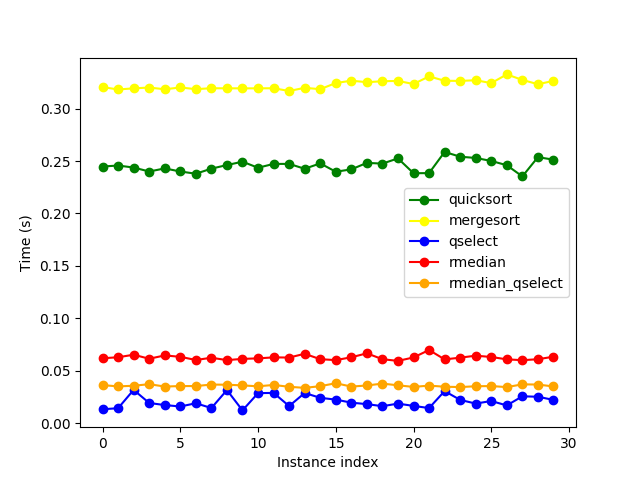
\includegraphics[scale=0.6]{../img/experiment_adhoc.png}
    \centering
    \caption{Computing time of the algorithms using the ad hoc instances}
    \label{fig:adhoc}
\end{figure}

\begin{figure}[htbp]
    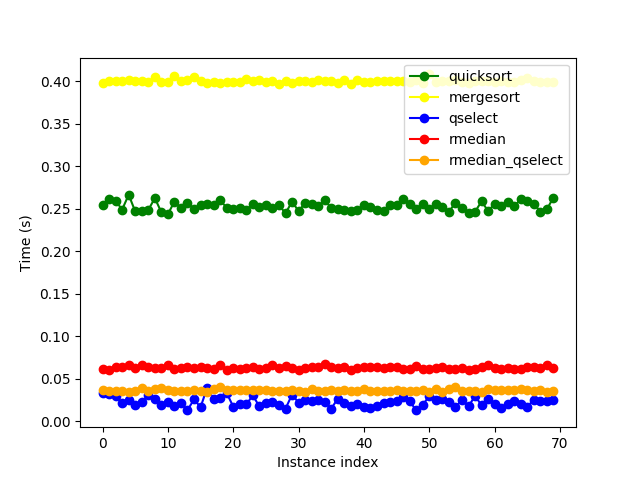
\includegraphics[scale=0.6]{../img/experiment_basic.png}
    \centering
    \caption{Computing time of the algorithms using the totally random instances}
    \label{fig:random}
\end{figure}

\section{Complexity plots}
I extended the \code{src/experiment.py} script to plot the complexity of each algorithm. In order to do that, I created 100 new totally random instances of increasing $n$ (from 1000 to 100000, with steps of 1000) and I run the experiment. Here you have the resultant plot (see figure \ref{fig:complexity}).

\begin{figure}[htbp]
    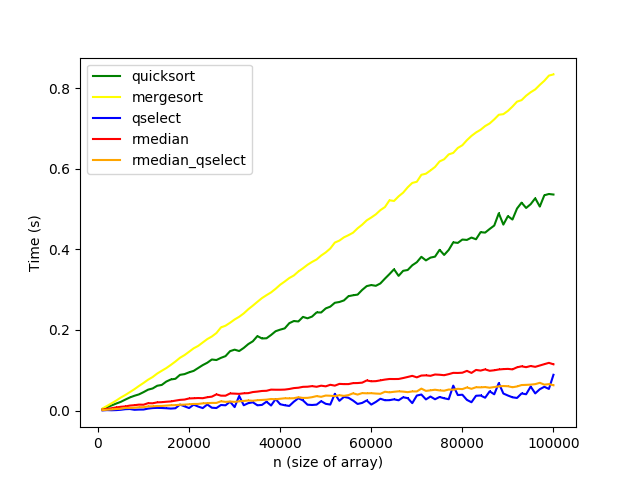
\includegraphics[scale=0.8]{../img/experiment_complexity.png}
    \centering
    \caption{Complexity of the algorithms}
    \label{fig:complexity}
\end{figure}

\section{Conclusions}
From all the experiments, I can conclude that \textbf{QSelect} is the fastest algorithm to find the median of an array of numbers. It is also more polyvalent, because it can be used to find the $i$-th element of an unsorted array. Furthermore, if \textbf{RMedian} uses \textbf{QSelect}, it is obtained a faster algorithm than \textbf{RMedian} alone, in some cases even better than \textbf{QSelect}. I want to mention that, as you can see in all figures, the worst cases of \textbf{QSelect} need more or less the same times than in \textbf{RMedian-QSelect}. You can also see that the computing times of \textbf{QSelect} and \textbf{QuickSort} have more variance (specially when increasing $n$) than the others. This happens because the selection of the pivot is really important, so its correct or wrong selection flows into good or bad times, and it is random. Because all these things, and because it does not have significant variances, I can say that the more reliable algorithm is \textbf{RMedian-QSelect}.

\begin{thebibliography}{9}

    \bibitem{qselect} Wikipedia. \emph{QuickSelect}. [ONLINE] Available at: \url{https://en.wikipedia.org/wiki/Quickselect}

    \bibitem{mergesort} Wikipedia. \emph{MergeSort}. [ONLINE] Available at: \url{https://en.wikipedia.org/wiki/Merge_sort}

    \bibitem{slides} Josep Diaz. \emph{Concentration of a random variable around its
    mean}. [ONLINE] Available at: \url{http://www.lsi.upc.edu/~diaz/Concentration.pdf}

\end{thebibliography}



\end{document}